\chapter{联邦学习与隐私安全}
\label{chap:2}

\section{概略}

2016 年 Google 提出了 Federated Learning(联邦学习),能够让所有用户的手机「合作式」训练一个强大的模型,同时资料可以只要存在用户自己的手机中,维持了资料的隐私性,在这几年,随着隐私意识与法规的提升,Federated Learning 也受到了各大公司、研究机构的重视。要搞懂Federated Learning有两个必备的知识,其一为资料隐私,其二为分布式机器学习(Distributed Machine Learning),接下来分别简单介绍这两者,并介绍Federated Learning的研究问题与第一个演算法 FedAvg。


\section{资料隐私}

Google 在多年前推出一个服务,能够整合Google mail, map, calendar等应用的资讯,提供用户更自动化的服务,其意义在于,某人今天暑假想要到荷兰阿姆斯特丹远离都市生活看著名的风车村,从订好机票的那一个,信件中收到航空公司的确认信,同时 Google 用他的人工智慧系统从信件中也抓到了这个资讯,帮你把来回的机票时间标在 Google Calendar 上,并且把你下飞机后会搭的接驳车、想要居住的旅馆都标在 Google Maps 上,使用者不用再一个一个手动,Google一次帮你做好。虽然很方便,考虑到侵犯隐私时,可以快速想像另一个情景,今天 Google Map 同时也有使用者过去的用餐地点的资料,知道使用者喜欢吃什么、不喜欢吃什么,所以把使用者在阿姆斯特丹喜欢的餐厅全部都标出来推荐给你。而 Google 从使用者的搜寻纪录也知道使用者喜欢什么类型的景点,所以也帮使用者把在阿姆斯特丹的行程规划好。虽说 Google 贴心地安排了所有的行程,但也顺势地藉由 GPS 定位或是搜寻纪录,投放了周边商家的广告,在无形之中旅游行程的客制化与人们的隐私权之间的界线开始变得更模糊了。也许可以稍微反思,当人们的定位或搜寻纪录被利用在投放广告等其他用途的同时,是不是也代表着人们的隐私正在一点一滴的流失。

 另外客制化跟隐私的界线在于,客制化的前提是使用个人资料,问题是哪些资料可以被使用,哪些不可以被使用,被如何使用,应该要能由使用者决定。 2018 年纽约时报揭露,剑桥分析公司使用 5000 万个 Meta 上用户的资料进行建模,进而研究出每个用户的个性、偏好,进而应用在 Psychographic Targeting (心理变数行销),针对每个人最容易被煽动的角度客制化行销文宣,进而影响大选结果。同时 2019 年 Netflix 将这个事件改编成短影集「个资风暴:剑桥分析事件」,引起了大众对个人资料在网路上流通的重视度。而 2020 年哈佛大学社会心理学教授 Shoshana Zuboff 出版了「监控资本主义时代(The Age of Surveillance Capitalism: The Fight for a Human Future at the New Frontier of Power)」,讲解了在高度数位化、智能化的现在,企业如何使用个人资料来改变使用者的行为。

 
这一系列的事件其实都显示出了,公众意识到了随着科技快速发展,现有法规对个人资料的保护已经不够完整。所幸在 2016 年欧盟就率先制定了GDPR (General Data Protection Regulation) 来限制企业对个人资料 (Personal Data) 的使用,订立出了一个高标准要求企业,GDPR 的核心是「给用户自由选择资料是否被使用」,包含了「被遗忘权」 (Right to be forgotten)、「限制处理权」(Right to restriction of processing),而 GDPR 的出现也冲击了现今最火热的两大技术「深度学习」、「区块链」。随着越来越高的隐私意识,深度学习研究者们也相对应的开启了 Privacy ML 的研究热潮,而 Federated Learning 的核心就是为了保有隐私,让用户在「不用上传自己资料到企业端的同时可以训练模型、使用智能化服务」。

\section{分布式机器学习}

分布式机器学习的本质就是 Distributed System (分布式系统) 跟机器学习的结合。而分布式系统的想法,其实就像是 GPU 的逻辑,当一个程式先后要做的很多工作,分摊给多个处理器、多台电脑来进行运算,那分工合作的结果就应该要缩短时间,得到更快速的结果。但是在分布式系统大家最大的困难其实是如何让不同台机器能够「相互沟通(Communication)」,假设今天我写了一个程式来运算 Mergesort,演算法的课程让我们知道我们可以在多个电脑中分别去一部份资料的 Mergesort,最后再 Merge 起来,但是问题是:怎么把每台电脑资料快速、稳定的传输到其他电脑。

 而沟通 (Communication) 是分布式系统的核心瓶颈,就像是类似于大学在做团体报告的时候,为了让每个人的编辑状况能够同步,人们会使用 Google doc、Google Slides、Google Spreadsheet...等共编软体,来同步每个人的进度。但是在过去这些软体不发达的时候,人们能做的就是用 Word 做好自己的部分,然后用随身碟带到出去传到别人电脑里再进行整合。在以前只能用随身碟来传输档案,而从某人家到组员家需要 2 小时车程,那这个沟通瓶颈就会让我觉得「还不如自己把报告做完」,因为 2 小时的通讯时间实在太久了。所以很多时候分布式系统会像通识课程一样,分组比不分组还忙。而 Federated Learning 其实就是让每个用户用自己的装置进行训练,得出「个人小模型」,训练结果再统整到云端上,统整出一个「多用户通用大模型」,借此用户可以保有自己资料不用上传,同时又可以享受到智能化服务。而 Federated Learning 核心困难也是如何让沟通的成本变得尽量低。
 
\section{联邦学习}

\begin{figure}[htb]
\centering 
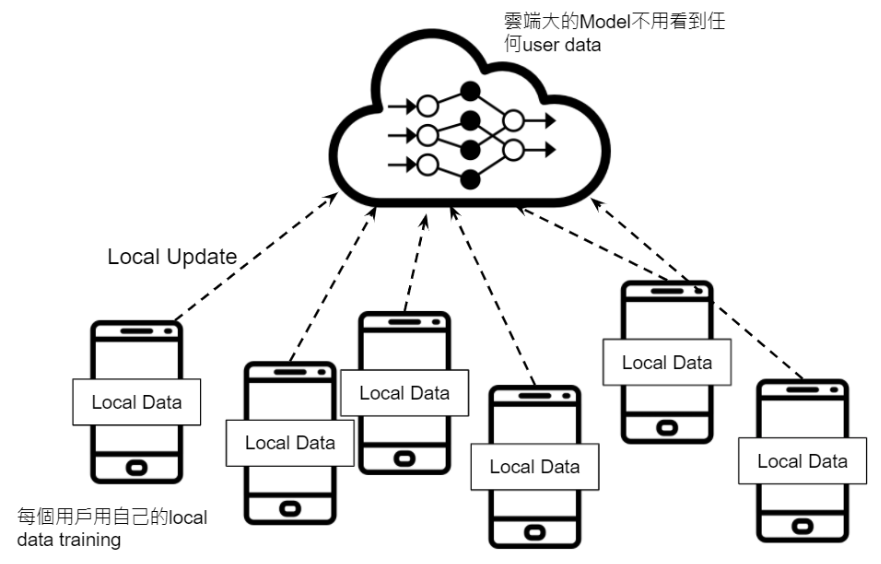
\includegraphics[width=0.70\textwidth]{img/newch2m1.png} 
\caption{联邦学习架构}
\label{Test}
\end{figure}

联邦学习的四个特点如下 :

\begin{itemize}
\item [-] 用户不用上传资料到云端,只要把资料存在自己装置中
\item [-] 每个用户在自己装置上进行训练
\item [-] 训练完后把跟资料无关的性质 (像是 Model Weight) 上传至云端,云端再统整大模型
\item [-] 期望这样训练的结果跟把所有用户资料统整起来一起训练的结果差不多。
\end{itemize}

而这个第 4 点其实就是论文中最常提到的公式 : 

\begin{equation}
\left|V_{F E D}-V_{S U M}\right|<\delta
\end{equation}

$V_{FED}$代表用 Federated Learning 训练出来的 Performance,$V_{SUM}$代表用传统方法,也就是所有资料上传云端所训练出来的 Performance,两者差距要够小。这边如果对应分布式机器学习此就是 Data Parallelism。而 Data Parallelism 也有四个特性如下 : 

\begin{itemize}
\item [-] 把资料打散分送给各台机器 (Client)
\item [-] 在 Client 端用初始的模型权重 (Model Weight) 算出一次 SGD 的 Gradient
\item [-] 每台 Client 把 Gradient 送回 Server
\item [-] Server 拿多台电脑送来的 Gradient 来更新 Weight
\end{itemize}

因为 Deep Learning 主要的运算瓶颈是在算出 Gradient,所以在这步我们进行大量平行,而用 Gradient 去更新 Weight 很快,所以交由 Server 一个来做,所以 Data Parallelism 可以大幅度提升训练速度。 Federated learning 其实的确就是一种特殊的 Data Parallelism,但是比起 Data Parallelism 有多 4 个特点如下。

\begin{itemize}
\item [-] Federated Learning 假设 Data 是 Non IID (Independent and identically distributed),因为每个用户装置上是用户各自的资料,而 Data Parallelism 还是一样先收集资料再「打散」给各个机器,所以 Non IID 是 Federated Learning 一个很核心的困境
\item [-] Federated Learning 给每个用户自主权,随时要离开 Federated Learning 的群体都可以离开,也避免了 User 突然断线对 Federated Learning 的影响,Distributed Learning 则是因为中央维护机器 Cluster,所以预期每一台机器都顺畅运作。
\item [-] Data Imbalance,因为 Training 主要是在用户端完成,所以我们不能藉由 Resample、调整 Learning Curve 来解决 Imbalance。
\item [-] 大规模分布,比起一般 Data Parallelism,Federated Learning 希望达成更大规模的平行。
\end{itemize}

同时因为用户端的沟通成本更高,随意一个现在的模型动辄就 2 至 3GB 的大小,如果很频繁的沟通,会占据用户的网路频宽,所以会希望更大幅度的减少沟通次数,用运算换沟通。

\section{FedAvg}

2016 年 Google 发表了 Federated learning of deep networks using model averaging 这篇论文,为 Federated Learning 奠定了研究方向。而论文里面也提出了第一个 Federated Learning 的演算法 FedAvg。其 FedAvg 的逻辑其实就是从 Data Parallelism 出发,再更进一步去减少沟通次数,而为了减少沟通次数,FedAvg 让每个装置进行多次的更新才沟通。每个用户装置 Update 多个 Batch后,得到新的 Model Weight,再把多个用户的 Model平均起来。因为每个用户都 Update 多个 Batch,所以得到的都是更「成熟」的模型,只需要沟通较少次就能得到好的模型。详情可以看演算法 Pseudocode。但是因为 NonIID 的特质,每个「成熟」的模型可能长相差异极大,所以 FedAvg 实际上需要更多的运算才能收敛好,但是只要减少沟通次数就是最终的胜利。

\begin{figure}[htb]
\centering 
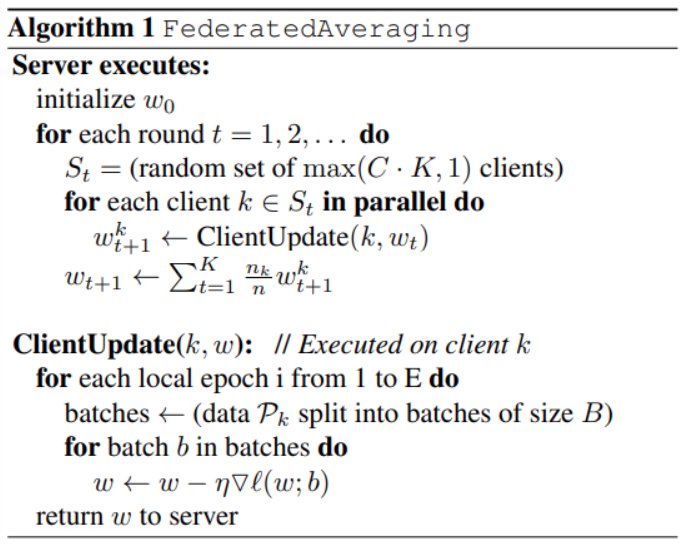
\includegraphics[width=0.70\textwidth]{img/newch2m2.png} 
\caption{伪代码}
\label{Test}
\end{figure}

\section{Federated Learning 分类}

从初始的 FedAvg 被提出后,研究者后来进而提出了 Federated Learning 的 3 种分类如下

\subsection{Horizontal Federated Learning (横向联邦学习)}

每个 Client 的资料有相同的「Feature Set (特征集)」,而彼此之间比较少用户重叠,实际上我前面讲的 Federated Learning 准确都是在讲 Horizontal Federated Learning。

包含 Google 的 FedAvg 可以让每个用户手机不上传你的讯息资料到云端上依旧训练出一个好的模型。同时像多个医疗机构也可以在不共用病患个资的前提下结合多家医院的模型来得到更精准的模型。

\begin{figure}[htb]
\centering 
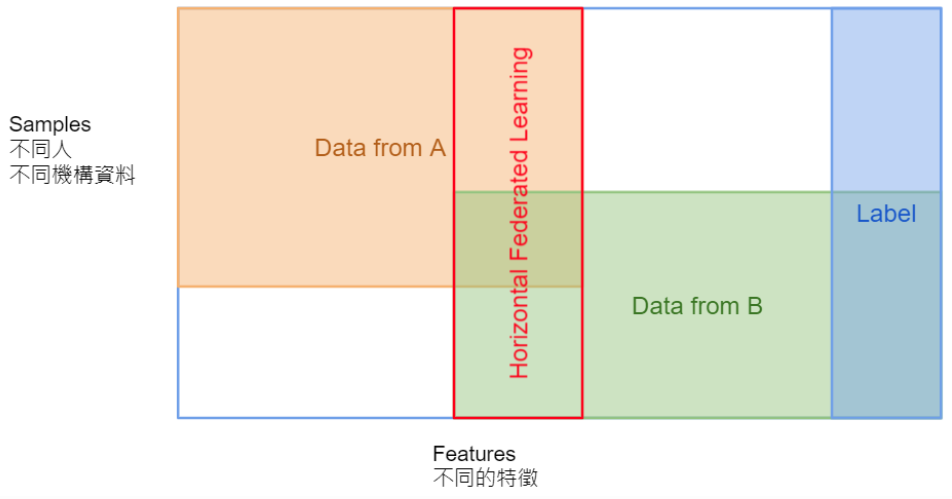
\includegraphics[width=0.70\textwidth]{img/newch2m3.png} 
\caption{Horizontal Federated Learning (横向联邦学习)}
\label{Test}
\end{figure}


\subsection{Vertical Federated Learning (纵向联邦学习)}

每个 Client 比较少重复的 Feature Set (特征集),但是会有大比例重叠的用户,像是一个地区的医疗机构跟政府机关可能面对的用户都是同一群用户,但是医疗机构的资料上可能以病历为主,政府机关则是以公民资料为主,里面有一部份特征重叠,但是更多是没有重叠的特征,这种时候就不能使用以往的 Data Parallelism 训练方法。先假设我们把所有资料都收集到云端上,这种时候我们可以用资料中那些重叠的特征,去对齐来自于不同机构的资料,这不是大问题,但是这在 Federated Learning 的设定下就做不到了,因此 Vertical Federated Learning 更多是使用特征加密的方法来保护用户隐私。

\begin{figure}[htb]
\centering 
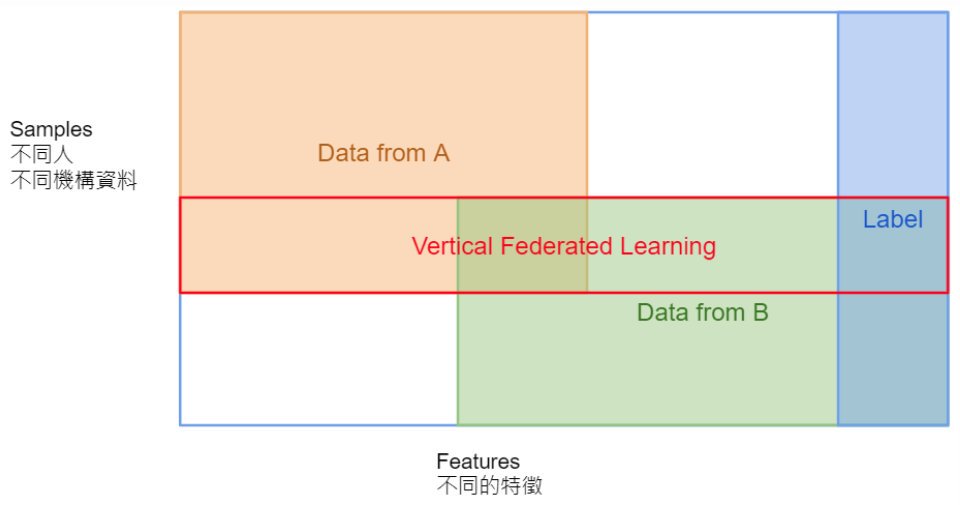
\includegraphics[width=0.70\textwidth]{img/newch2m4.png} 
\caption{Vertical Federated Learning (纵向联邦学习)}
\label{Test}
\end{figure}

\subsection{Federated Transfer Learning (联邦迁移学习)}

如果 Client 之间 Feature Set (特征集)跟用户都重叠较少,那就属于 Federated Transfer Learning,训练的难度也急遽上升,目前也还是一个非常初期的研究领域。

可以看到除了最基础的 Horizontal Federated Learning 以外,其他两种 Federated Learning 的应用场景也非常复杂,但是如果能够达成利用任意机构的资料都能提升模型 Performance,甚至用户跟 Feature set (特征集)都没有重叠,那就能同时保有每个机构资料的隐密性,又更进一步提升人工智能的威力。

\begin{figure}[htb]
\centering 
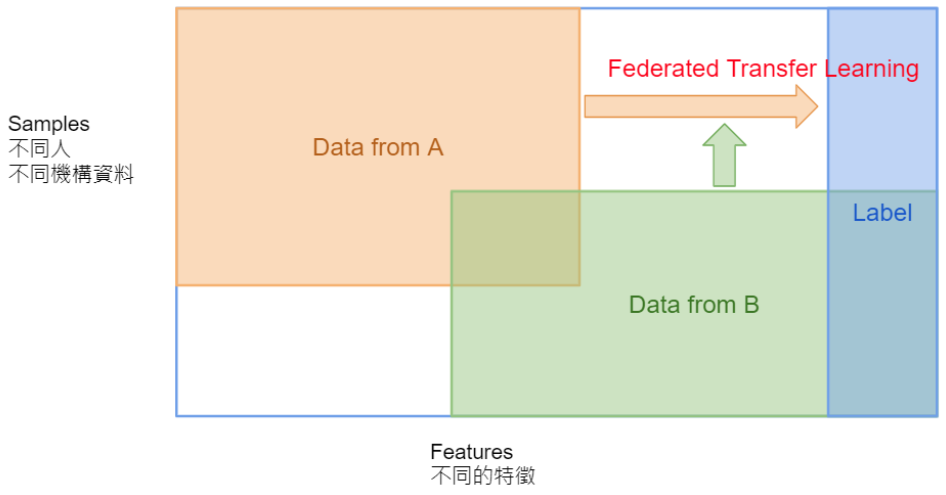
\includegraphics[width=0.70\textwidth]{img/newch2m5.png} 
\caption{Federated Transfer Learning (联邦迁移学习)}
\label{Test}
\end{figure}

\section{Federated Learning 困境}

Federated Learning 有很多研究的困难点,这边提几个常被讨论的观点如下

\begin{itemize}
\item [-] 隐私真的有被保护的部分可以看到 Federated Learning 把非 Data 的资讯上传到云端,可能是 Gradient 可能是 weight,但是这些资讯其实都是由 Data 得出,乍看之下没有侵犯用户隐私,但是多个研究都显示可以只从 Gradient 或是 Weight 得出每个用户资料的某些特性,还是泄漏了用户隐私。
\item [-] 公平 VS 隐私,Imbalance 的问题在 Federated Learning 一直都很难解,Train 出来的模型大多都有某种偏见,这些偏见又无法消弭掉,那我们的模型如何公平,公平与隐私在 Federated Learning 的设定下好像就变成了两难。
\item [-] 难以抵抗攻击,在 Robustness 跟 Attack 这块我们知道可以藉由传送一些有害的 Gradient 或是在训练集加入有害的资料来让 Model 烂掉,这在 Federated Learning 里面更难解决,因为我们不知道这个用户的资料是特别不同,还是他刻意在攻击我们的模型
\end{itemize}